\documentclass{beamer}
\usepackage{graphicx, tabularx}
\usetheme{Singapore}

\def\UrlBreaks{\do\/\do-} % URL breaks
\setbeamertemplate{caption}[numbered] % number figures
\setbeamertemplate{bibliography item}{\insertbiblabel} % bibliography numbers
\makeatletter
\newcommand*{\rom}[1]{\expandafter\@slowromancap\romannumeral #1@}
\makeatother

\title{Research Project Last-Layer Variational Inference}
\author{Philipp von Bachmann}
\institute{University of Tübingen}
\date{\today}



\begin{document}
        \begin{frame}
            \titlepage
        \end{frame}
        
        \section{Recap}
        \begin{frame}
            \frametitle{Where we left of}
            \begin{columns}
                \begin{column}{0.5\textwidth}
                    \begin{itemize}
                        \item Setup: Deep Learning, learn weight distribution with Variational Inference
                        \item Use Gaussian distributions for prior and variational
                        \item Initally good results for Regression and mixed results for Classification
                    \end{itemize}
                \end{column}
                \begin{column}{0.5\textwidth}
                    \begin{figure}
                        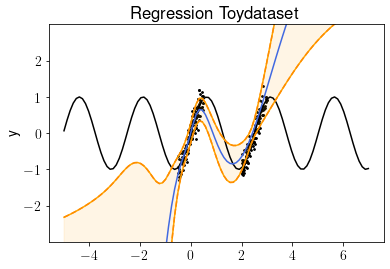
\includegraphics[width=\textwidth]{images/Regression/Toydataset.png}
                    \end{figure}
                \end{column}
            \end{columns}
        \end{frame}
        
        \section{Closed-form Solutions}
        \begin{frame}
            \frametitle{Regression}
            \begin{itemize}
                \item Expected log-likelihood $\mathbb{E}_{q_{\phi}(\theta)}[\log{p(y \vert f_{\theta}(x))}]$ has a closed-form solution in the Regression case
                \item Loss function becomes more stable compared to Monte-Carlo sampling
                \item Leads to faster convergence
            \end{itemize}
            \begin{figure}
                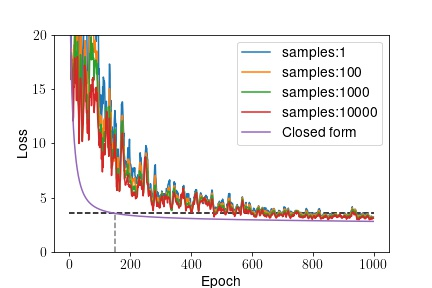
\includegraphics[width=0.7\textwidth]{images/Regression/CFvsMC.jpg}
            \end{figure}
        \end{frame}

        \begin{frame}
            \frametitle{Classification}
            \begin{itemize}
                \item No closed-form solution, but multiple approximations exist
                \item However, they perform worse than Monte-Carlo sampling
                \item Possible explanation: MC introduces noise which acts as a Reguralizer
            \end{itemize}
            \begin{figure}
                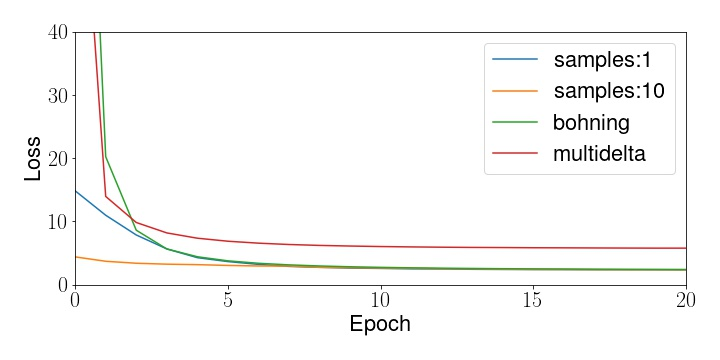
\includegraphics[width=0.7\textwidth]{images/Classification/CFvsMC.jpg}
            \end{figure}
        \end{frame}
        
        \section{Last-Layer vs Full Layer VI}
        \begin{frame}
            \frametitle{Overview}
            Advantages of Last-Layer
            \begin{itemize}
                \item Scale better with network size
                \item Closed-form solutions or approximations for the log-likelihood available
                \item Prediction is faster because of closed-form (Regression) or easy approximations (Classification, Probit)
            \end{itemize}
            Disadvantages
            \begin{itemize}
                \item Not all parameters are treated Bayesian
                \item Less complex, could therefore underfit
            \end{itemize}
        \end{frame}


        \begin{frame}
            \frametitle{Regression}
            \begin{columns}
                \begin{column}{0.6\textwidth}
                \begin{itemize}
                    \item Use closed-form for Last-Layer versus single sample MC for Full-Layer training
                    \item Full-Layer has better solution, especially higher in-between uncertainty
                    \item Last-Layer training and predicting is faster
                \end{itemize}
                \begin{figure}
                    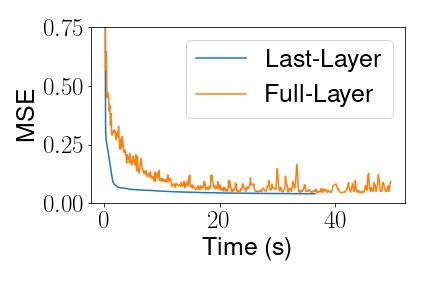
\includegraphics[width=0.8\textwidth]{images/Regression/LLvsFullMSE.jpg}
                \end{figure}
                \end{column}
                \begin{column}{0.4\textwidth}
                    \begin{figure}
                        \vspace*{-2cm}
                        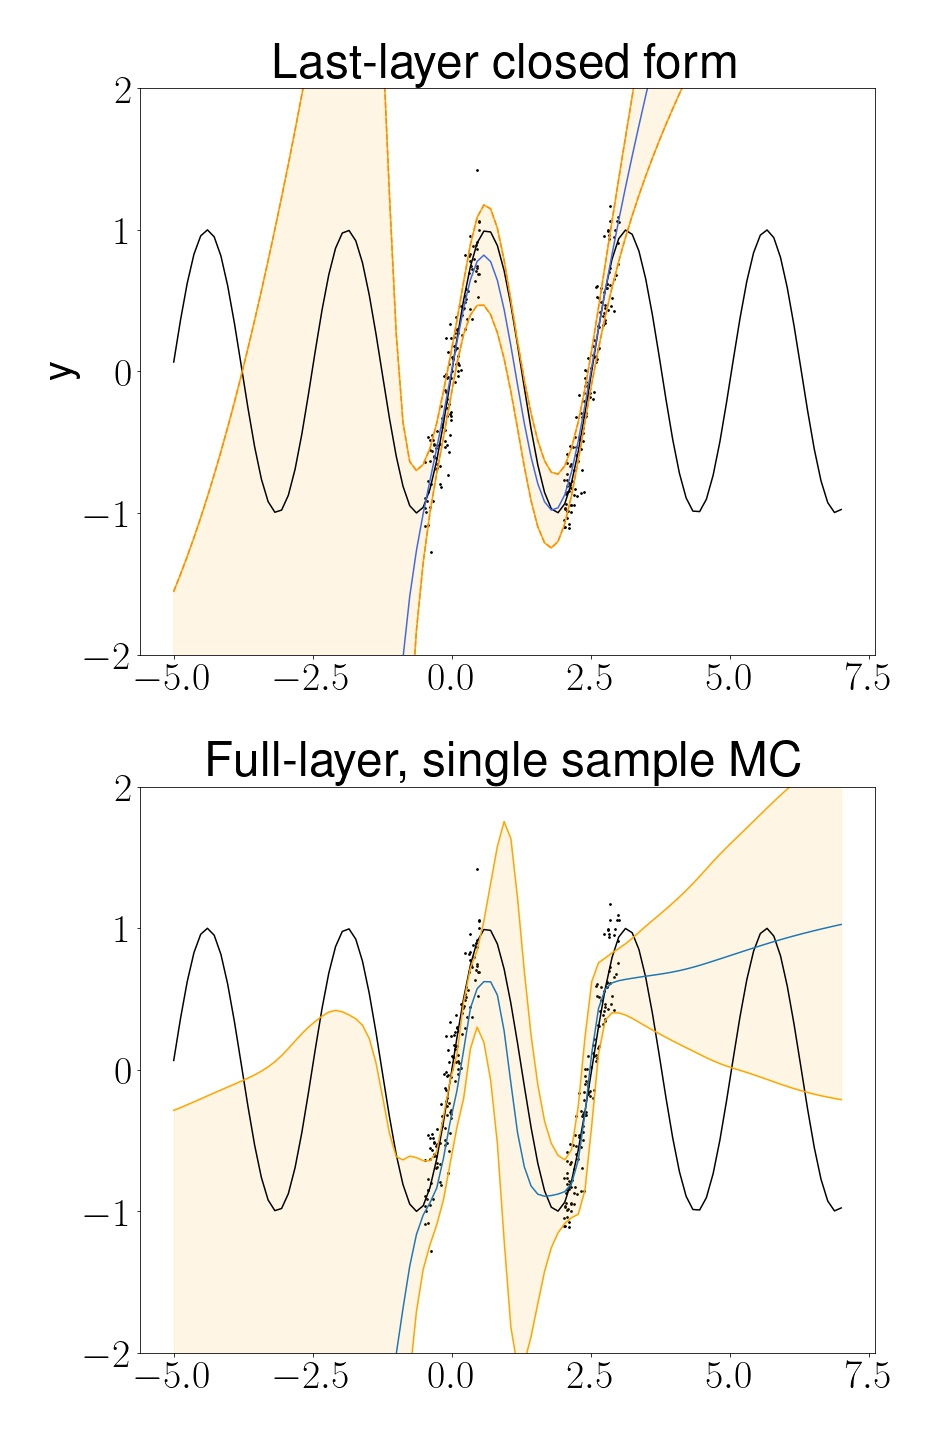
\includegraphics[height=0.8\textheight]{images/Regression/LLvsFull.jpg}
                    \end{figure}
                \end{column}
            \end{columns}
        \end{frame}

        \begin{frame}
            \frametitle{Classification: MNIST}
            \begin{itemize}
                \item Last-Layer training is faster in the case of classification
                \item Performance is similar
            \end{itemize}
            \begin{columns}
                \begin{column}{0.5\textwidth}
                    \begin{figure}
                        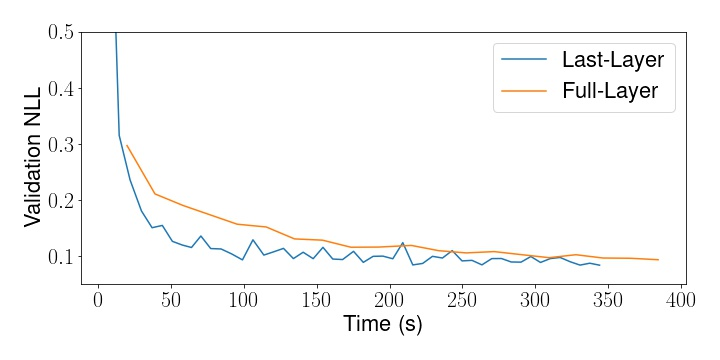
\includegraphics[width=1.1\textwidth]{images/Classification/LLvsFull2.jpg}
                    \end{figure}                  
                \end{column}
                \begin{column}{0.5\textwidth}                
                    \begin{tabular}{p{0.5\textwidth}|p{0.2\textwidth}|p{0.2\textwidth}}
                        Mean confidence\\ (in \%)&Full-Layer & Last-Layer\\
                        \hline
                        Test dataset & 93.4 & 95.5\\
                        OOD dataset & 67.8 & 70.1
                    \end{tabular}
                \end{column}
            \end{columns}
        \end{frame}


        \section{VI vs Laplace}

        \begin{frame}
            \frametitle{Equivalence of VI and Laplace}
            \begin{itemize}
                \item Claim: Laplace approximation is equivalent to Natural Gradient Descent for VI
                \item Bayesian Learning Rule which can be derived from VI:     
                    \begin{equation}
                        \lambda_{t+1} \leftarrow \lambda_{t} - \rho \tilde{\nabla}_\lambda E_{q_t}[L(\theta) - H(q_t)]
                    \end{equation}
                    where $\lambda$ natural parameters, $\tilde{\nabla}$ natural gradient, $L$ Loss and $H$ Entropy
                \item If $q = \mathcal{N}(m, S^{-1})$, the update for precision $S$ becomes:
                    \begin{equation}
                        S_{t+1} = (1 - \rho_t) S_t + \rho_t E_{q_t}[\nabla^2_\theta L(\theta)]
                    \end{equation}
                \item Equivalent to online-computation of the Hessian
            \end{itemize}
        \end{frame}

        \begin{frame}
            \frametitle{Laplace initialization}
            \begin{columns}
                \begin{column}{0.5\textwidth}
                    \begin{itemize}
                        \item Idea: Use Laplace approximation as initialization for VI
                        \item Scenarios:
                            \begin{itemize}
                                \item Pretrained networks
                                \item Speed up training
                            \end{itemize}
                        \item Result: Laplace approximation provides good initialization 
                    \end{itemize}    
                \end{column}
                \begin{column}{0.5\textwidth}                    
                    \begin{figure}
                        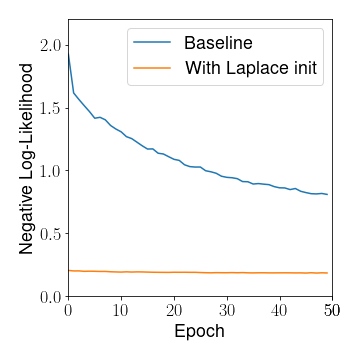
\includegraphics[width=\textwidth]{images/Classification/LaplaceInit.png}
                    \end{figure}
                    % \begin{tabular}{cccc}
                    %     &laplace & vilaplace & virefined \\
                    %     test & 91.9 & 93.2 & 51.5 \\
                    %     ood & 67.8 & 69.6 & 36.8
                    % \end{tabular}
                \end{column}
            \end{columns}
        \end{frame}
        
        


        % \begin{frame}
        %     \frametitle{Regression}
        %     add regression comparison of kernels here
        %     \begin{figure}
        %         \includegraphics[width=0.8\textwidth]{images/Regression/FullCov.jpg}
        %     \end{figure}
        % \end{frame}

        % \begin{frame}
        %     \frametitle{Classification: Two Moons}
        %     add non-bayesian vs best kernel comparison here, maybe vs laplace?
        %     \begin{columns}
        %         \column{0.5\textwidth}
        %         \begin{figure}
        %             \includegraphics[width=\textwidth]{images/TowMoons/Baseline.jpg}
        %         \end{figure}
        %         \column{0.5\textwidth}
        %         \begin{figure}
        %             \includegraphics[width=\textwidth]{images/TowMoons/Diagonal.jpg}
        %         \end{figure}
        %     \end{columns}
        % \end{frame}








\end{document}

% TODO:
- all plots hline
- complete Advantages
- make plot cf for classification
- make plot init for laplace
